  \section{Comparison of Solver Concepts}
  
     \subsection{Convergence Behaviour on Locally Refined Block Structured Grids with Different Degrees of Coupling}

      Show how the implicit treatment of block boundaries maintains (high) convergence rates. Plot Residual over number of iterations. Plot Wall time for a single block using SIP, KSP, COUPLED for different grid resolutions.

\subsection{Parallel Performance}

In many cases scientific code is used to solve complex problems regarding memory requirements, on the other side results have to be made available in short time. In both scenarios code that is able to run in parallel can alleviate the present problems. Code that runs in parallel can allocate more memory resources which makes the calculation of complex problems feasible. If the code is scalable the program execution can be shortened by using more processors to solve a problem of constant size.

The solver framework that has been developed in the curse of the present thesis has been parallelized using the PETSc library. After introducing the used hardware and software, the central measures of parallel performance are presented. Then preliminary test results using low-level benchmarks are performed, which establish upper performance bounds on the parallel efficiency and the scalability of the developed solver framework. The results of the efficiency evaluation is presented in the last subsections.
\subsubsection{Employed Hardware and Software -- The Lichtenberg-High Performance Computer }

All performance analyses that are presented in this thesis were conducted on the Lichtenberg-High Performance Computer, also known as \emph{HHLR} (\emph{Hessischer Hochleistungsrechner}) \cite{hhlr}. The cluster consist of different sections according to the used hardware. Throughout the thesis tests were performed using the first and the second mpi section of the cluster. The first section consists of 705 nodes of which each runs two Intel\textregistered Xeon\textregistered E5-2670 processors and offers 32GB of memory. The second section consists of 356 nodes of which each runs two Intel Xeon E5-2680 v3 processors and offers 64GB of memory. The interconnect for both sections uses a FDR-14 InfiniBand.

All tests programs were compiled using the Intel compiler suite version 15.0.0 and the compiler options
\begin{lstlisting}
-O3 -xHost
\end{lstlisting}
As mpi implementation openmpi version 1.8.2 was chosen. The PETSc framework version 3.5.3 was configured using the options
\begin{lstlisting}
--with-blas-lapack-dir=/shared/apps/intel/2015/composer_xe_2015/mkl/lib/intel64/ \
--with-mpi-dir=/shared/apps/openmpi/1.8.2_intel \
COPTFLAGS="-O3 -xHost" FOPTFLAGS="-O3 -xHost" \
CXXOPTFLAGS="-O3 -xHost" \
--with-debugging=0 \
--download-hypre \
--download-ml
\end{lstlisting}

\subsubsection{Measures of Performance}
\begin{itemize}
\item Maße definieren
\item Nochmal Hager,Wellein studieren
\item Guidelines for measuring performance (bias through system processes or user interaction), only measure calculation time do not consider I/O in the beginning and the end
\item Cite Schäfer and Peric with their different indicators for parallel efficiency, load balancing and numerical efficiency
\end{itemize}

\subsubsection{Preliminary Upper Bounds on Performance -- The STREAM Benchmark}

Scientific applications that solve partial differential equations rely on sparse matrix computations, which usually exhibit the sustainable memory bandwidth as bottleneck with respect to the runtime performance of the program \cite{hager11}. The purpose of this section is to establish a frame in terms of an upper bound on performance in which the efficiency developed solver framework can be evaluated critically. As common measure for the maximum sustainable bandwidth, low-level benchmarks can be used, which focus on evaluating specific properties of the hardware architecture to be used. In this case the STREAM benchmark suite provides apt tests, which are designed to work with data sets that exceed the cache size of the involved processor architecture. This forces the processors to stream the needed data directly from the memory instead of reusing the data residing in their caches. These types of tests can be used to calculate an upper bound on the memory bandwidth.

In terms of parallel scalability, the STREAM benchmark can also be used as an upper performance bound. According to \cite{petsc-web-page} the parallel performance of memory bandwidth limited codes correlates with the parallel performance of the STREAM benchmark, i.e. a scalable increase in memory bandwidth is necessary for scalable application performance. The intermediate results of the benchmark can then be used to test different configurations that bind hardware resources to the involved processes. Before presenting results the different binding configurations will be explained.

The first configuration sequentially binds the processes to the cores beginning on the first socket. When every core has a bound process the binding algorithm binds the following processes to cores of the second socket. The second configuration binds the processes in a round robin manner regarding the sockets. This configuration in difference to the second configuration binds one process to three cores. Figures \ref{fig:binding1},\ref{fig:binding2} and \ref{fig:binding3} demonstrate the different binding options for two sockets and processors with twelve cores each, when 8 processes are to be bound to the resources.

\begin{figure}[h]
  \centering
  \label{fig:binding1}
    \input{./img/map2.tikz.tex}
    \centering{}
  \caption{Default binding using openmpi on anode with two sockets and processors with each twelve cores}
\end{figure}

\begin{figure}[h]
  \centering
  \label{fig:binding2}
    \newcommand*{\xMin}{0}%
\newcommand*{\xMax}{12}%
\newcommand*{\yMin}{0}%
\newcommand*{\yMax}{1}%
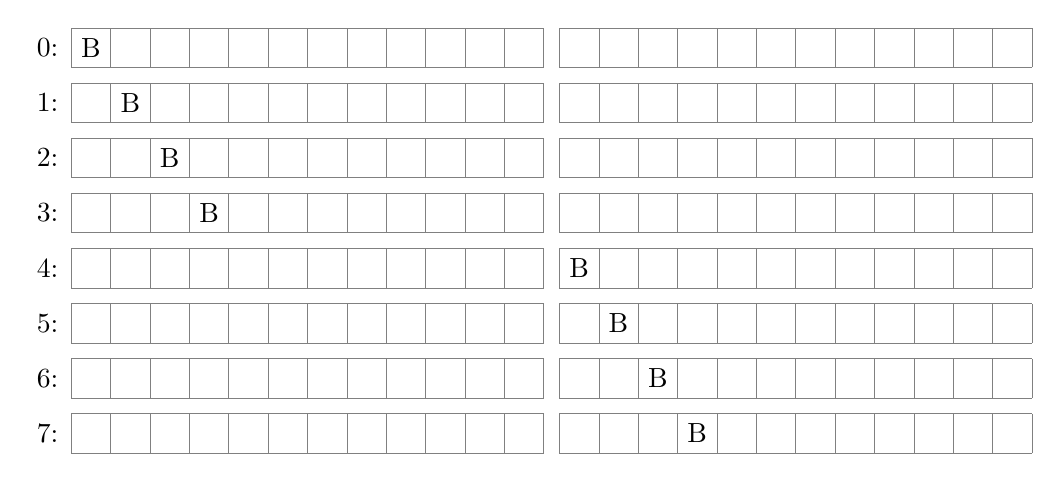
\begin{tikzpicture}
%   \foreach \i in {\xMin,...,\xMax} {
%       \draw [very thin,gray] (\i,\yMin) -- (\i,\yMax)  ;
%   }
%   \foreach \i in {\yMin,...,\yMax} {
%       \draw [very thin,gray] (\xMin,\i) -- (\xMax,\i) ;
%   }
    \foreach \j in {0,0.7,1.4,2.1,2.8,3.5,4.2,4.9} {
    \foreach \i in {0,0.5,1.0,1.5,2.0,2.5,3.0,3.5,4.0,4.5,5.0,5.5,6.0} {
        \draw [very thin,gray] (\i,\j) -- (\i,\j+0.5)  ;
        }

    \foreach \i in {\j,\j+0.5} {
        \draw [very thin,gray] (0,\i) -- (6.0,\i)  ;
        }


    \foreach \i in {0,0.5,1.0,1.5,2.0,2.5,3.0,3.5,4.0,4.5,5.0,5.5,6.0} {
        \draw [very thin,gray] (\i+6.2,\j) -- (\i+6.2,\j+0.5)  ;
        }

    \foreach \i in {\j,\j+0.5} {
        \draw [very thin,gray] (6.2,\i) -- (12.2,\i)  ;
        }
    }

    \node at (-0.3,0.25) {7: };
    \node at (-0.3,0.95) {6: };
    \node at (-0.3,1.65) {5: };
    \node at (-0.3,2.35) {4: };
    \node at (-0.3,3.05) {3: };
    \node at (-0.3,3.75) {2: };
    \node at (-0.3,4.45) {1: };
    \node at (-0.3,5.15) {0: };
    \node at (0.25,5.15) {B};
    \node at (0.75,4.45) {B};
    \node at (1.25,3.75) {B};
    \node at (1.75,3.05) {B};
    \node at (0.25+6.2,2.35) {B};
    \node at (0.75+6.2,1.65) {B};
    \node at (1.25+6.2,0.95) {B};
    \node at (1.75+6.2,0.25) {B};

  

\end{tikzpicture}

    \centering{}
  \caption{Process binding using openmpi and map-by ppr:8:node map-by ppr:4:socket on a node with two sockets and processors with each twelve cores}
\end{figure}


\begin{figure}[h]
  \centering
  \label{fig:binding3}
    \input{./img/map3.tikz.tex}
    \centering{}
  \caption{Process binding using openmpi and map-by ppr:8:node map-by ppr:4:socket:PE=3 on a node with two sockets and processors with each twelve cores}
\end{figure}

        Pinning of processes (picture), preliminary constraints by hardware and operating systems, identification of bottlenecks and explain possible workarounds, history and results of STREAM. Bandwidth as Bottleneck, how to calculate a Speedup estimate based on the measured bandwidth. PETSc Implementation of STREAM

\begin{figure} \centering
  \pgfplotsset{every axis/.append style={
      font=\large,
      line width=1pt,
  tick style={line width=0.8pt}}}
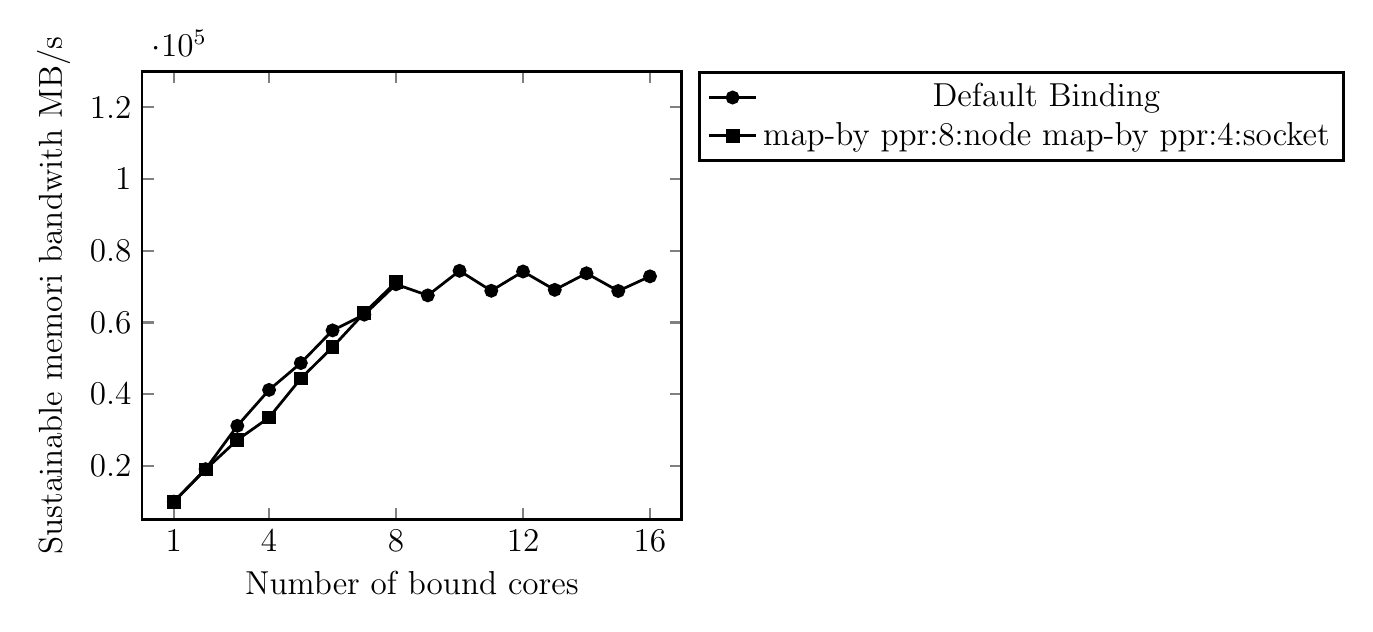
\begin{tikzpicture}
\begin{axis}[
    ylabel={Sustainable memori bandwith MB/s},
    xlabel={Number of bound cores},
    xtick={1,4,8,12,16},
    %ytick={1.7e-003,1.75e-3,1.8e-003,1.85e-3},
    %yticklabels={1.7E-3,1.75E-3,1.8E-3,1.85E-3},
    %ymin=1.65e-003,ymax=1.9e-003,
    xmin=0,xmax=17,
    ymin=0.5e4,ymax=1.3e5,
    legend pos=outer north east,
    %height=20cm,width=10cm
    ]
    \addplot[color=black,mark=*] coordinates {
        (1,10056.2733)
        (2,19114.3429)
        (3,31197.8399)
        (4,41210.0612)
        (5,48699.7232)
        (6,57803.5686)
        (7,62187.9785)
        (8,70658.3730)
        (9,67558.4259)
        (10,74413.8457)
        (11,68849.0631)
        (12,74223.3175)
        (13,69109.0762)
        (14,73729.0608)
        (15,68784.2613)
        (16,72872.4480) };
        \addlegendentry{Default Binding};
    \addplot[color=black,mark=square*] coordinates {
        (1 ,10044.2323)
        (2 ,19036.1755)
        (3 ,27258.6888)
        (4 ,33509.0570)
        (5 ,44386.9342)
        (6 ,53130.5978)
        (7 ,62695.4511)
        (8 ,71295.7113) };
        \addlegendentry{map-by ppr:8:node map-by ppr:4:socket}
\end{axis}
\end{tikzpicture}
\caption{Sustainable memory bandwidth for the STREAM benchmark (Triad) for different binding options on MPI1}
\end{figure}

\begin{figure} \centering
  \pgfplotsset{every axis/.append style={
      font=\large,
      line width=1pt,
  tick style={line width=0.8pt}}}
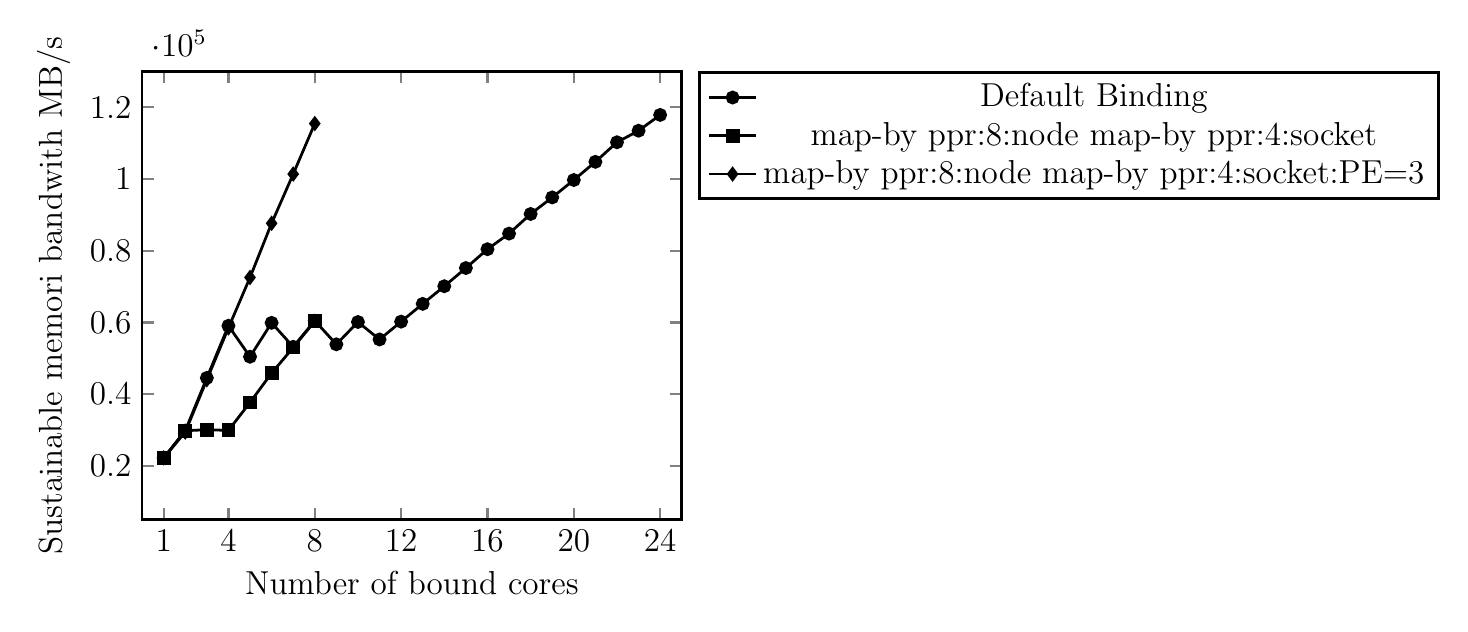
\begin{tikzpicture}
\begin{axis}[
    ylabel={Sustainable memori bandwith MB/s},
    xlabel={Number of bound cores},
    xtick={1,4,8,12,16,20,24},
    %ytick={1.7e-003,1.75e-3,1.8e-003,1.85e-3},
    %yticklabels={1.7E-3,1.75E-3,1.8E-3,1.85E-3},
    %ymin=1.65e-003,ymax=1.9e-003,
    legend pos=outer north east,
    xmin=0,xmax=25,
    ymin=0.5e4,ymax=1.3e5,
    %height=20cm,width=10cm
    ]
    \addplot[color=black,mark=*] coordinates {
           
      (1, 22201.8738 )
      (2,    29846.0651 )
      (3,    44558.8130 )
      (4,    59096.4718 )
      (5,    50460.8297 )
      (6,    59912.1938 )
      (7,    53222.7910 )
      (8,    60491.6764 )
      (9,    53922.4875 )
      (10,    60144.1732 )
      (11,    55273.7403 )
      (12,    60248.1185 )
      (13,    65200.5600 )
      (14,    70118.7250 )
      (15,    75192.3175 )
      (16,    80439.8917 )
      (17,    84793.6761 )
      (18,    90263.9931 )
      (19,    94881.4421 )
      (20,    99735.0136 )
      (21,   104804.3772 )
      (22,   110256.7754 )
      (23,   113478.3185 )
    (24,   117880.3816 ) };
     \addlegendentry{Default Binding};
     \addplot[color=black,mark=square*] coordinates{
       (1, 22211.6717)
       (2, 29836.1141)
       (3, 30113.6704)
       (4, 29919.5219)
       (5, 37713.7578)
       (6, 45888.1496)
       (7, 53019.1276)
     (8, 60375.4338) };
     \addlegendentry{map-by ppr:8:node map-by ppr:4:socket};
     \addplot[color=black,mark=diamond*] coordinates{
       (1, 22265.7147)
       (2, 29467.1111)
       (3, 44064.6918)
       (4, 58503.9143)
       (5, 72560.6185)
       (6, 87667.8368)
       (7,101388.5503)
     (8,115464.4300) };
     \addlegendentry{map-by ppr:8:node map-by ppr:4:socket:PE=3};
\end{axis}
\end{tikzpicture}
\caption{Sustainable memory bandwidth for the STREAM benchmark (Triad) for different binding options on MPI1}
\end{figure}

      \subsubsection{Discussion of Results for Parallel Efficiency}
      \subsubsection{Speedup Measurement for Analytic Test Cases}

    \subsection{Test Cases with Varying Degree of Non-Linearity}
      
      As Peric says I want to prove that the higher the non-linearity of NS, the better relative convergence rates can be achieved with a coupled solver. Fi

      \subsubsection{Transport of a Passive Scalar -- Forced Convection}
      \subsubsection{Buoyancy Driven Flow -- Natural Convection}
      \subsubsection{Flow with Temperature Dependent Density -- A Highly Non-Linear Test Case}
        Maybe I could consider two test cases, one with oscillating density and one with a quadratic polynomial. Interesting would be also to consider the dependence of convergence on another scalar transport equation

    \subsection{Realistic Testing Scenarios -- Benchmarking}
        Also consider simple load balancing by distributing matrix rows equally
      
      \subsubsection{Flow Around a Cylinder 3D -- Stationary}
        Describe Testing Setup (Boundary conditions and grid). Present results and compare them with literature.
      \subsubsection{Flow Around a Cylinder 3D -- Instationary}
        \begin{itemize}
          \item\url{http://www.featflow.de/en/benchmarks/cfdbenchmarking/flow/dfg_flow3d/dfg_flow3d_configuration.html}
        \end{itemize}
        Describe Testing Setup (Boundary conditions and grid). Present results and compare them with literature.

      \subsubsection{Heat-Driven Cavity Flow}
        \begin{itemize}
          \item \url{http://www.featflow.de/en/benchmarks/cfdbenchmarking/mit_benchmark.html}
        \end{itemize}
        Describe Testing Setup (Boundary conditions and grid). Present results and compare them with literature.
    \subsection{Realistic Testing Scenario -- Complex Geometry}
